\chapter{Privacy Filters}
\label{cha:privacy-filters}
As discussed in the previous chapter, the goal of this chapter is to find a solution to the information leakage problems that come with data aggregation in Solid, and with requesting resources in general. This problem arises due to the fact no distinction is made between the trust level given to client applications. These applications either get the full resource (when they have the necessary authorization), or they don't get the resource at all. However, since mostly structured data is handled by Solid, it should be possible to restrict which parts of a resource are exposed and allow more granular access control (i.e., within a resource).

As illustrated by figure \ref{fig:privacy-utility-tradeoff}, improved privacy always comes with a trade-off regarding data utility. Evidently, data with less or less precise attribute values will be more private, but this same property also renders the data less useful. Making this trade-off is very context-dependent (how much is the application trusted, what kind of data is requested etc.). As such, rendering data more private must happen dynamically, at the time of a request, such that details of the request can be taken into account when determining what transformations ought to happen.

\begin{figure}[h]
    \centering
    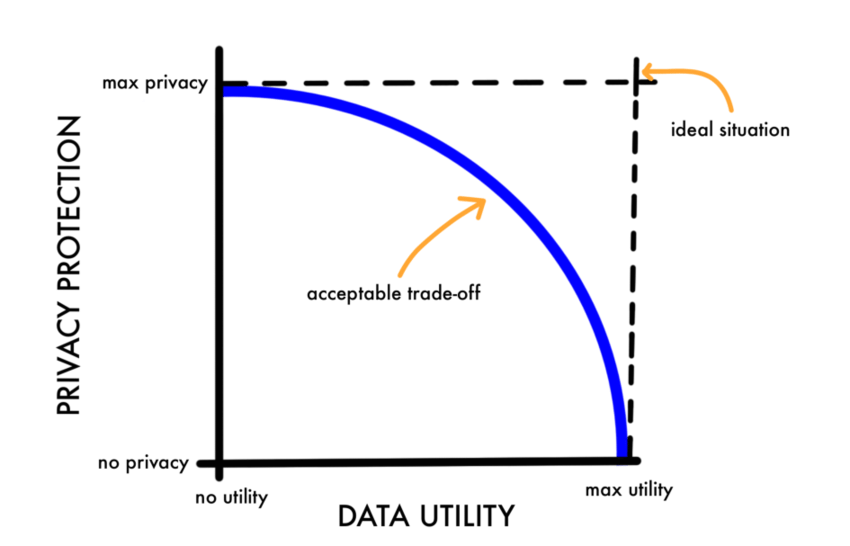
\includegraphics[width=0.8\textwidth]{images/privacy-filter/Data-Privacy-Protection-versus-Data-Utility.png}
    \caption{Illustration of the privacy-utility trade-off, from \citet{datasharing-implications}}
    \label{fig:privacy-utility-tradeoff}
\end{figure}

\noindent This chapter introduces the concept of \textit{privacy filters}, which dynamically strip away attributes of exposed data in accordance with some predefined rules. A prototype that implements privacy filters is developed for the \gls{CSS} as a part of \middleware{}. This specific component is called \mwprivacy{} (short for Privacy-enhancing Plugin for Solid Applications). However, since it forms a part of the complete middleware, the specific implementation will hereafter also be referenced to as \middleware{}. This implementation provides a middleware in the Solid server which provides more fine-grained privacy control options. 

In the developed prototype privacy filters are represented by a JSON document (per data scheme), describing which transformations ought to happen to which data attribute. Users can then specify how much privacy they want (in general, or for specific data types). When a request is received, \middleware{} checks what data type it is and what level of privacy the user has requested. Subsequently, a number of transformations are applied to the data (as specified by the privacy filter configuration file), after which the transformed data is returned to the application. An example of what such a rewrite can look like is provided in figure \ref{fig:example-treatment-privacy-filter}.

\begin{figure}[H]
\centering
\begin{subfigure}{.5\textwidth}
  \centering
  \begin{minted}[linenos,tabsize=2,breaklines]{json}
{
"accountOwner": "Jesse Geens",
"IBAN": "BE66123456783456",
"saldo": 665.53,
"currency": "EUR",
"history": [
    {
    "from": "BE17954824458821",
    "to": "BE66123456783456",
    "from_name": "Mark Jansen",
    "to_name": "Jesse Geens",
    "amount": 33.7,
    "timestamp": 1645447425,
    "description": "Payback borrowed money"
    }, {
    "from": "BE66123456783456",
    "to": "BE15954347627130",
    "from_name": "Jesse Geens",
    "to_name": "Steffie Smits",
    "amount": 10.0,
    "timestamp": 1645440365,
    "description": "Drinks"
    }
]}
  \end{minted}
  \caption{Data before applying privacy filter}
  \label{fig:data-before-privacy-filter}
\end{subfigure}%
\begin{subfigure}{.5\textwidth}
  \centering
  \begin{minted}[linenos,tabsize=2,breaklines]{json}
{
"accountOwner": "J.G.",
"IBAN": "BE42429824824354",
"saldo": 712.1171,
"currency": "EUR",
"history": [
    {
    "from": "BE17954824458821",
    "to": "BE42429824824354",
    "from_name": "Mark Jansen",
    "to_name": "J.G.",
    "amount": 34.8,
    "timestamp": 1645440000,
    "description": "Payback borrowed money"
    }, {
    "from": "BE42429824824354",
    "to": "BE15954347627130",
    "from_name": "J.G.",
    "to_name": "Steffie Smits",
    "amount": 9.45,
    "timestamp": 1645440000,
    "description": "Drinks"
    }
]}
  \end{minted}
  \caption{Data after applying privacy filter}
  \label{fig:data-after-privacy-filter}
\end{subfigure}
\caption{Example of data treatment by privacy filter, applied to financial transactions data}
\label{fig:example-treatment-privacy-filter}
\end{figure}

\newpage
\noindent The next sections discusses how \middleware{} was designed by listing the requirements that were envisioned before its development, followed by a detailed description of the subsequent design decisions and implementation details. Evaluation of the developed prototype is discussed in chapter \ref{cha:evaluation}.



\section{Privacy levels}
\label{sec:privacylevels}
\noindent In order to provide an intuitive mechanism for selecting which data is transformed, the concept of privacy levels is introduced. Privacy levels form an abstraction above the concrete data transformations and \gls{PETs} that are applied to the data before it is passed on to the application. This ensures that non-technical users can use a privacy-enhancing middleware, without needing to understand the technical details of the technologies and tactics that are employed. 

\middleware{} is configured with a default privacy level, but also supports specific privacy levels for certain data schemes. For example, a user could configure \middleware{} to use privacy level 2 by default, but privacy level 4 on bank transactions, since he does not want to expose this data. This makes the middleware more context-sensitive and allows for strong configurability. The privacy-utility trade-off can then also be taken into account for specific applications that need data with very high utility to deliver usable results. To make clear to the user what data is exposed an explanation should also be included (for every data type) which specifies concretely what will happen to the data under a certain privacy level.

Another important aspect is that the developers of privacy filters for specific data schemes must be aware of what privacy levels map to what leakage or tactics. This is best determined by privacy experts as it is a very complex topic. However, appendix \ref{appendix:privacy-levels} shows an example of such a mapping that was used to guide the development of configuration files for the prototype of \middleware{}.

\section{Implementation}

\middleware{} is implemented as an extension of the \acrlong{CSS}. The complete code and instructions can be found at \url{https://github.com/jessegeens/pepsa-component}.

\subsection{Design decisions}
In every architectural design, important decisions have to be made based on some sort of cost-benefit analysis: there is no free lunch. Similarly, this is the case with the design of \middleware{}. This section describes the reasoning behind a number of important design decisions that have been made during the modelling and development.

\subsubsection{Positioning}
A first important aspect of the design of \middleware{} is where it is logically positioned. There are two main possibilities, both with their own advantages. 

One possibility would be to make \middleware{} an extension of an existing Solid Server (such as, in our case, the \gls{CSS}). In this regard, it would be a true middleware. Furthermore, this would result in significantly sped up development, as well as much better performance. A disadvantage of this approach is that it leads to more centralization: if a user is using a pod provided by a third-party not running \middleware{}, there is no way to enable this. Extending an existing solid server also means choosing one specific server to support, making the solution incompatible with other servers.

The other possibility would be to build \middleware{} as a proxy. Requests from the Solid application would be directed to \middleware{} instead, which fetches the data, sanitizes it, and then replies with the sanitized data. This is a much less centralized option, but comes at a big performance cost. There are is more network usage and double the number of HTTP requests, for example. However, there is also a very important technical limitation. As was discussed in section \ref{sec:solid-oidc}, Solid uses \gls{DPoP} tokens. As can be seen in listing \ref{listing:dpop}, the \texttt{htu} parameter of the \gls{DPoP} token body prevents this token from being used in another pod, essentially making the proxy solution impossible when communicating with a Solid server using this authentication mechanism.

As such, the first option (extending an existing Solid server) is seen as the only possible choice. It also has the additional advantage of fulfilling another requirement. Since this is an extension of the Solid server and does not really interact with the Solid protocol itself, this extension is much easier to keep up-to-date with the quickly evolving Solid specification. Lastly, developing this as an extension of a Solid server also enables it to form a complete middleware when combined with the new access token mechanism.

\subsubsection{Supporting multiple data schemes}
Solid supports storing nearly any type of resource, both linked and non-linked. The data that is most prone to leakage in the context of a data aggregator is structured data. Structured data can take many forms, and any good middleware should be independent of the types of structured data that are requested or passing through it. However, \middleware{} needs to perform operations on the data that passes through it, and should thus have some context as to how it should handle a specific data scheme. Two possibilities for tackling this problem were envisioned.

A first possibility would be to have separate components, where each component is responsible for performing transformations on the input data of a specific data scheme. The components would be loaded dynamically at run-time, using dependency injection technology such as \textit{components.js}\footnote{\url{https://componentsjs.readthedocs.io/en/latest/}}. This would result in great flexibility: the transformation component can perform virtually any transformation. However, a first big disadvantage of this strategy is that it results in a significant development time for each component (and thus, for every supported data scheme). This can result in a lack of support for many (popular) data schemes, making \middleware{} significantly less useful. Another major downside is that this imposes new weaknesses from a security point-of-view, as untrusted code is imported in and executed on the Solid server.

A second option that was considered was to provide \middleware{} with an internal library of parsers for each content representation, which support a predefined set of transformations. For example, there would be a component that performs pseudonymization on data that is represented in JSON. At startup, the software would then read a number of configuration files, one for every supported data scheme. These files then specify how a data scheme should be detected, and what transformations ought to be applied to it. This requires more up-front coding to support this library of transformations for content representations. There is also a computational cost associated with having to parse all these configuration files and apply the rules expressed in them, instead of directly executing code. Despite these drawbacks, there is also a very large advantage to this approach: supporting new data schemes becomes a much easier and faster task. The only work that needs to be performed to support a new data scheme would be to write a scheme configuration file, something that can be done in a few hundred lines of JSON.

In the end, the second option was opted for. The reason for this is that the cost of writing new components specifically for one data scheme is too high for the relatively meager advantages it gives over the other approach. The appendix contains the JSON Schema used to describe such configuration files (see listing \ref{listing:privacy-filter-jsonschema}) as well as an example of such a scheme configuration file, specifically aimed at use case \ref{usecase:personal-finance} modifying financial data (see listing \ref{listing:privacy-filter-kbc}).

\begin{table}[H]
\begin{center}
\begin{tabulary}{\textwidth}{p{0.20\textwidth}p{0.8\textwidth}}
\textbf{Transformation name} & \textbf{Description}                                                                                                                                                          \\ \hline
Remove               & The targeted and deliberate omission of PII from the data record or data set.                                                                                                 \\
Pseudonym            & The systematic replacement of direct identifiers with surrogates, whereby the mapping between surrogate and identity is kept separately.                                      \\
Perturbation         & The insertion of randomized noise into the values of the data to hide exact values                                                                                 \\
Random               & Tactics that involve the modification of PII attribute values/records by injecting artificial random elements.                                                                \\
Encrypt              & Using cryptographic means to encode the PII attribute values / records / datasets.                                                                                            \\
Hash                 & Using cryptographic hash functions to obfuscate the PII attribute values / records / datasets in a deterministic fashion.                                                                                            \\
\end{tabulary}
\caption{Overview of data transformations supported in \middleware{}}
\label{table:supported-transformations}
\end{center}
\end{table}

\subsubsection{Supported transformations}
Table \ref{table:supported-transformations} gives an overview of which transformations are currently supported in \middleware{}. The choice for supported transformations is mostly based on the discussion from section \ref{sec:transformation-approaches}. This section discussed a taxonomy of architectural tactics involving data transformations. Some tactics could not be mapped to an equivalent tactic in our middleware because the middleware works on a per-request basis. An example of this is the \textit{Select / Filter} tactic, which keeps a copy of the original data. The \textit{Aggregate} tactic was not applicable as \middleware{} does not support grouping data elements, since data is treated on a per-attribute basis. Similar arguments hold for other tactics that are not supported. The \textit{Perturbation} tactic is based on the \textit{Blur} tactic from table \ref{table:de-id-taxonomy}, but renamed to convey its applicability to numeric values. Similarly, \textit{Encrypt} is supported along with the similar \textit{Hash} tactic.



\subsection{Implementation in CSS}
The implementation of \middleware{} is realised as an extension of the \acrlong{CSS}\footnote{\url{https://github.com/solid/community-server}}, leveraging components.js to substitute a component of the \gls{CSS} with a component provided by \middleware{}. An overview of the architecture of the \gls{CSS} is presented in figure \ref{fig:solid-arch}.

Concretely, the main component of \middleware{} is the \texttt{AnonymizingHTTPHandler}, which extends the \texttt{OperationHttpHandler} class provided by the \gls{CSS}. Using a custom components.js configuration, this new class is injected into the \gls{CSS} by giving it as an argument to the \texttt{ParsingHttpHandler}. On diagram \ref{fig:solid-arch}, this is located under \texttt{AuthenticatedLdpHandler}.

A configuration file for the \gls{CSS} specifying the dependency injection of the \texttt{AnonymizingHTTPHandler} can be found in the appendix, under listing \ref{listing:css-config}.

Figure \ref{fig:arch-overview} gives an overview of the system architecture of \middleware{}. Components that are part of a vanilla version of the \gls{CSS} are colored in blue. The red component, \texttt{AnonymizingHTTPHandler}, is the main component of the middleware and is the component that is injected into the \gls{CSS}. The yellow components are also included dynamically through the configuration file (listing \ref{listing:css-config}), such that other content representations can also easily be supported. The \texttt{ParserSelector} can then, based on the content representation that is defined in the detected data scheme, select the correct parser to perform the execution of all specified transformations. 
Figure \ref{fig:pepsa-sequence} illustrates the flow of how a privacy filter is applied to an incoming request in the \gls{CSS}.

\begin{sidewaysfigure}[h]
    \centering
    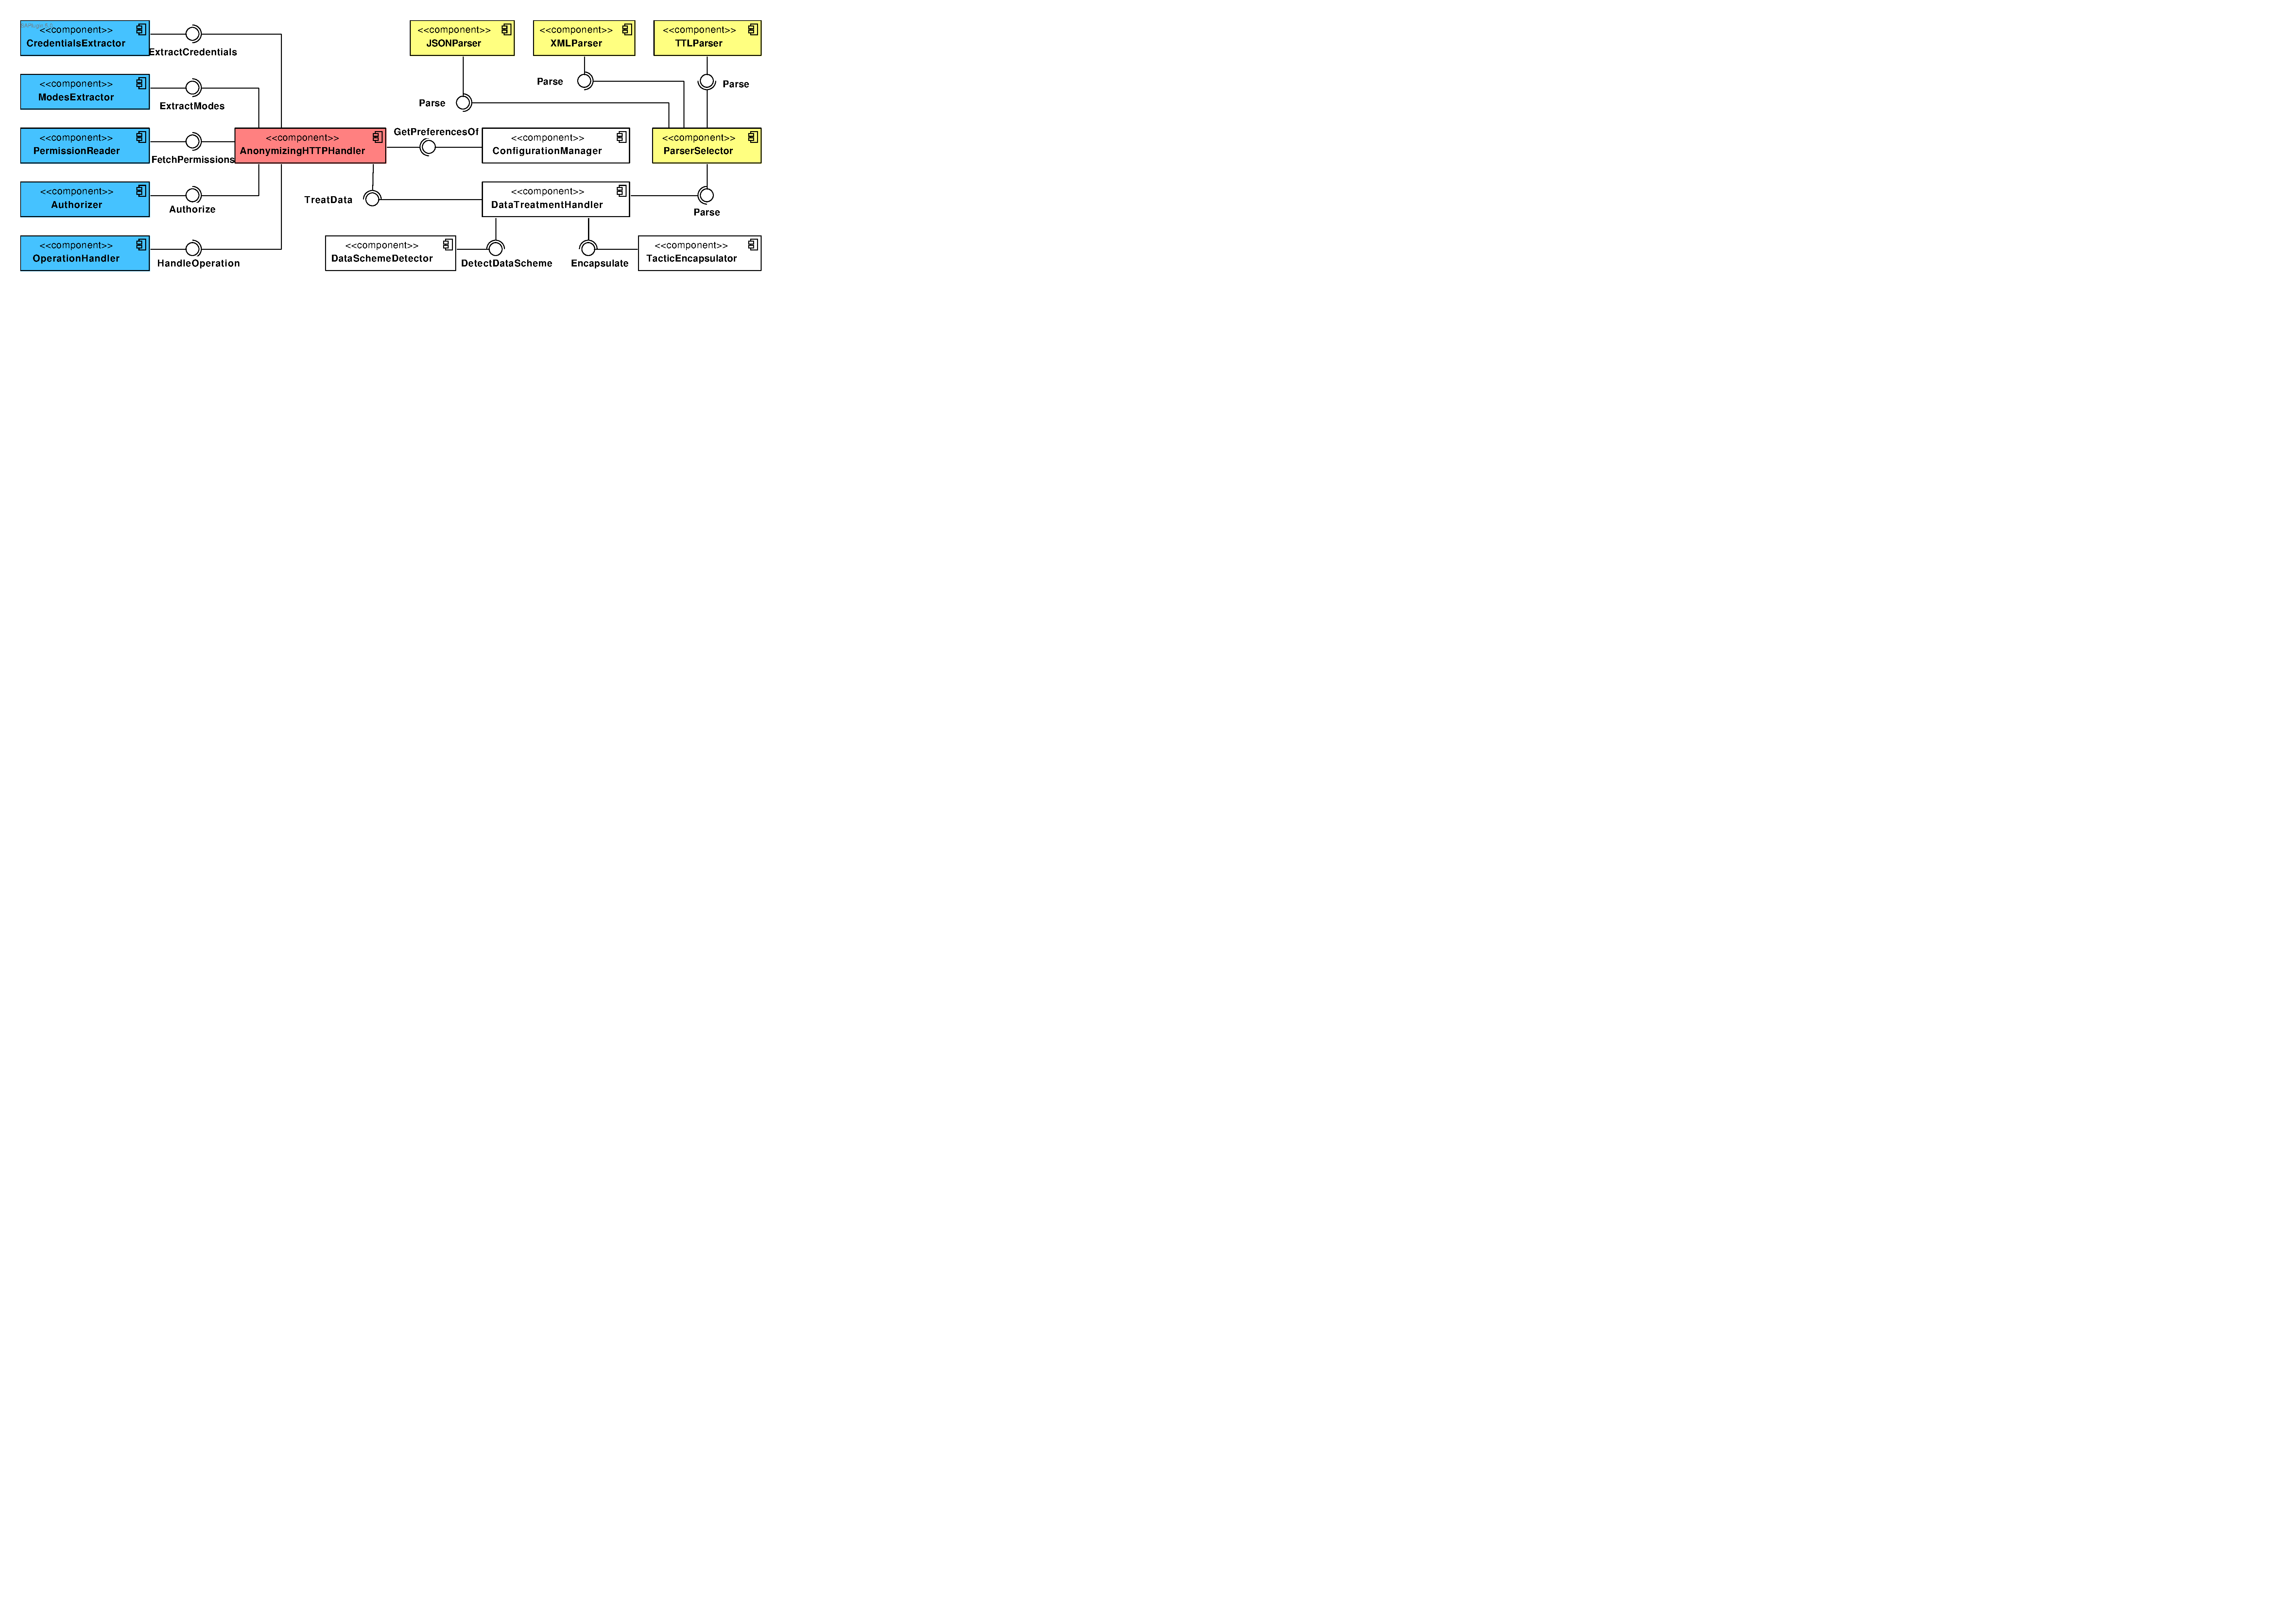
\includegraphics[width=1.0\textwidth]{images/architecture/PePSA-System-Overview.pdf}
    \caption{Overview of \middleware{} privacy filter architecture}
    \label{fig:arch-overview}
\end{sidewaysfigure}



\begin{sidewaysfigure}[h]
    \centering
    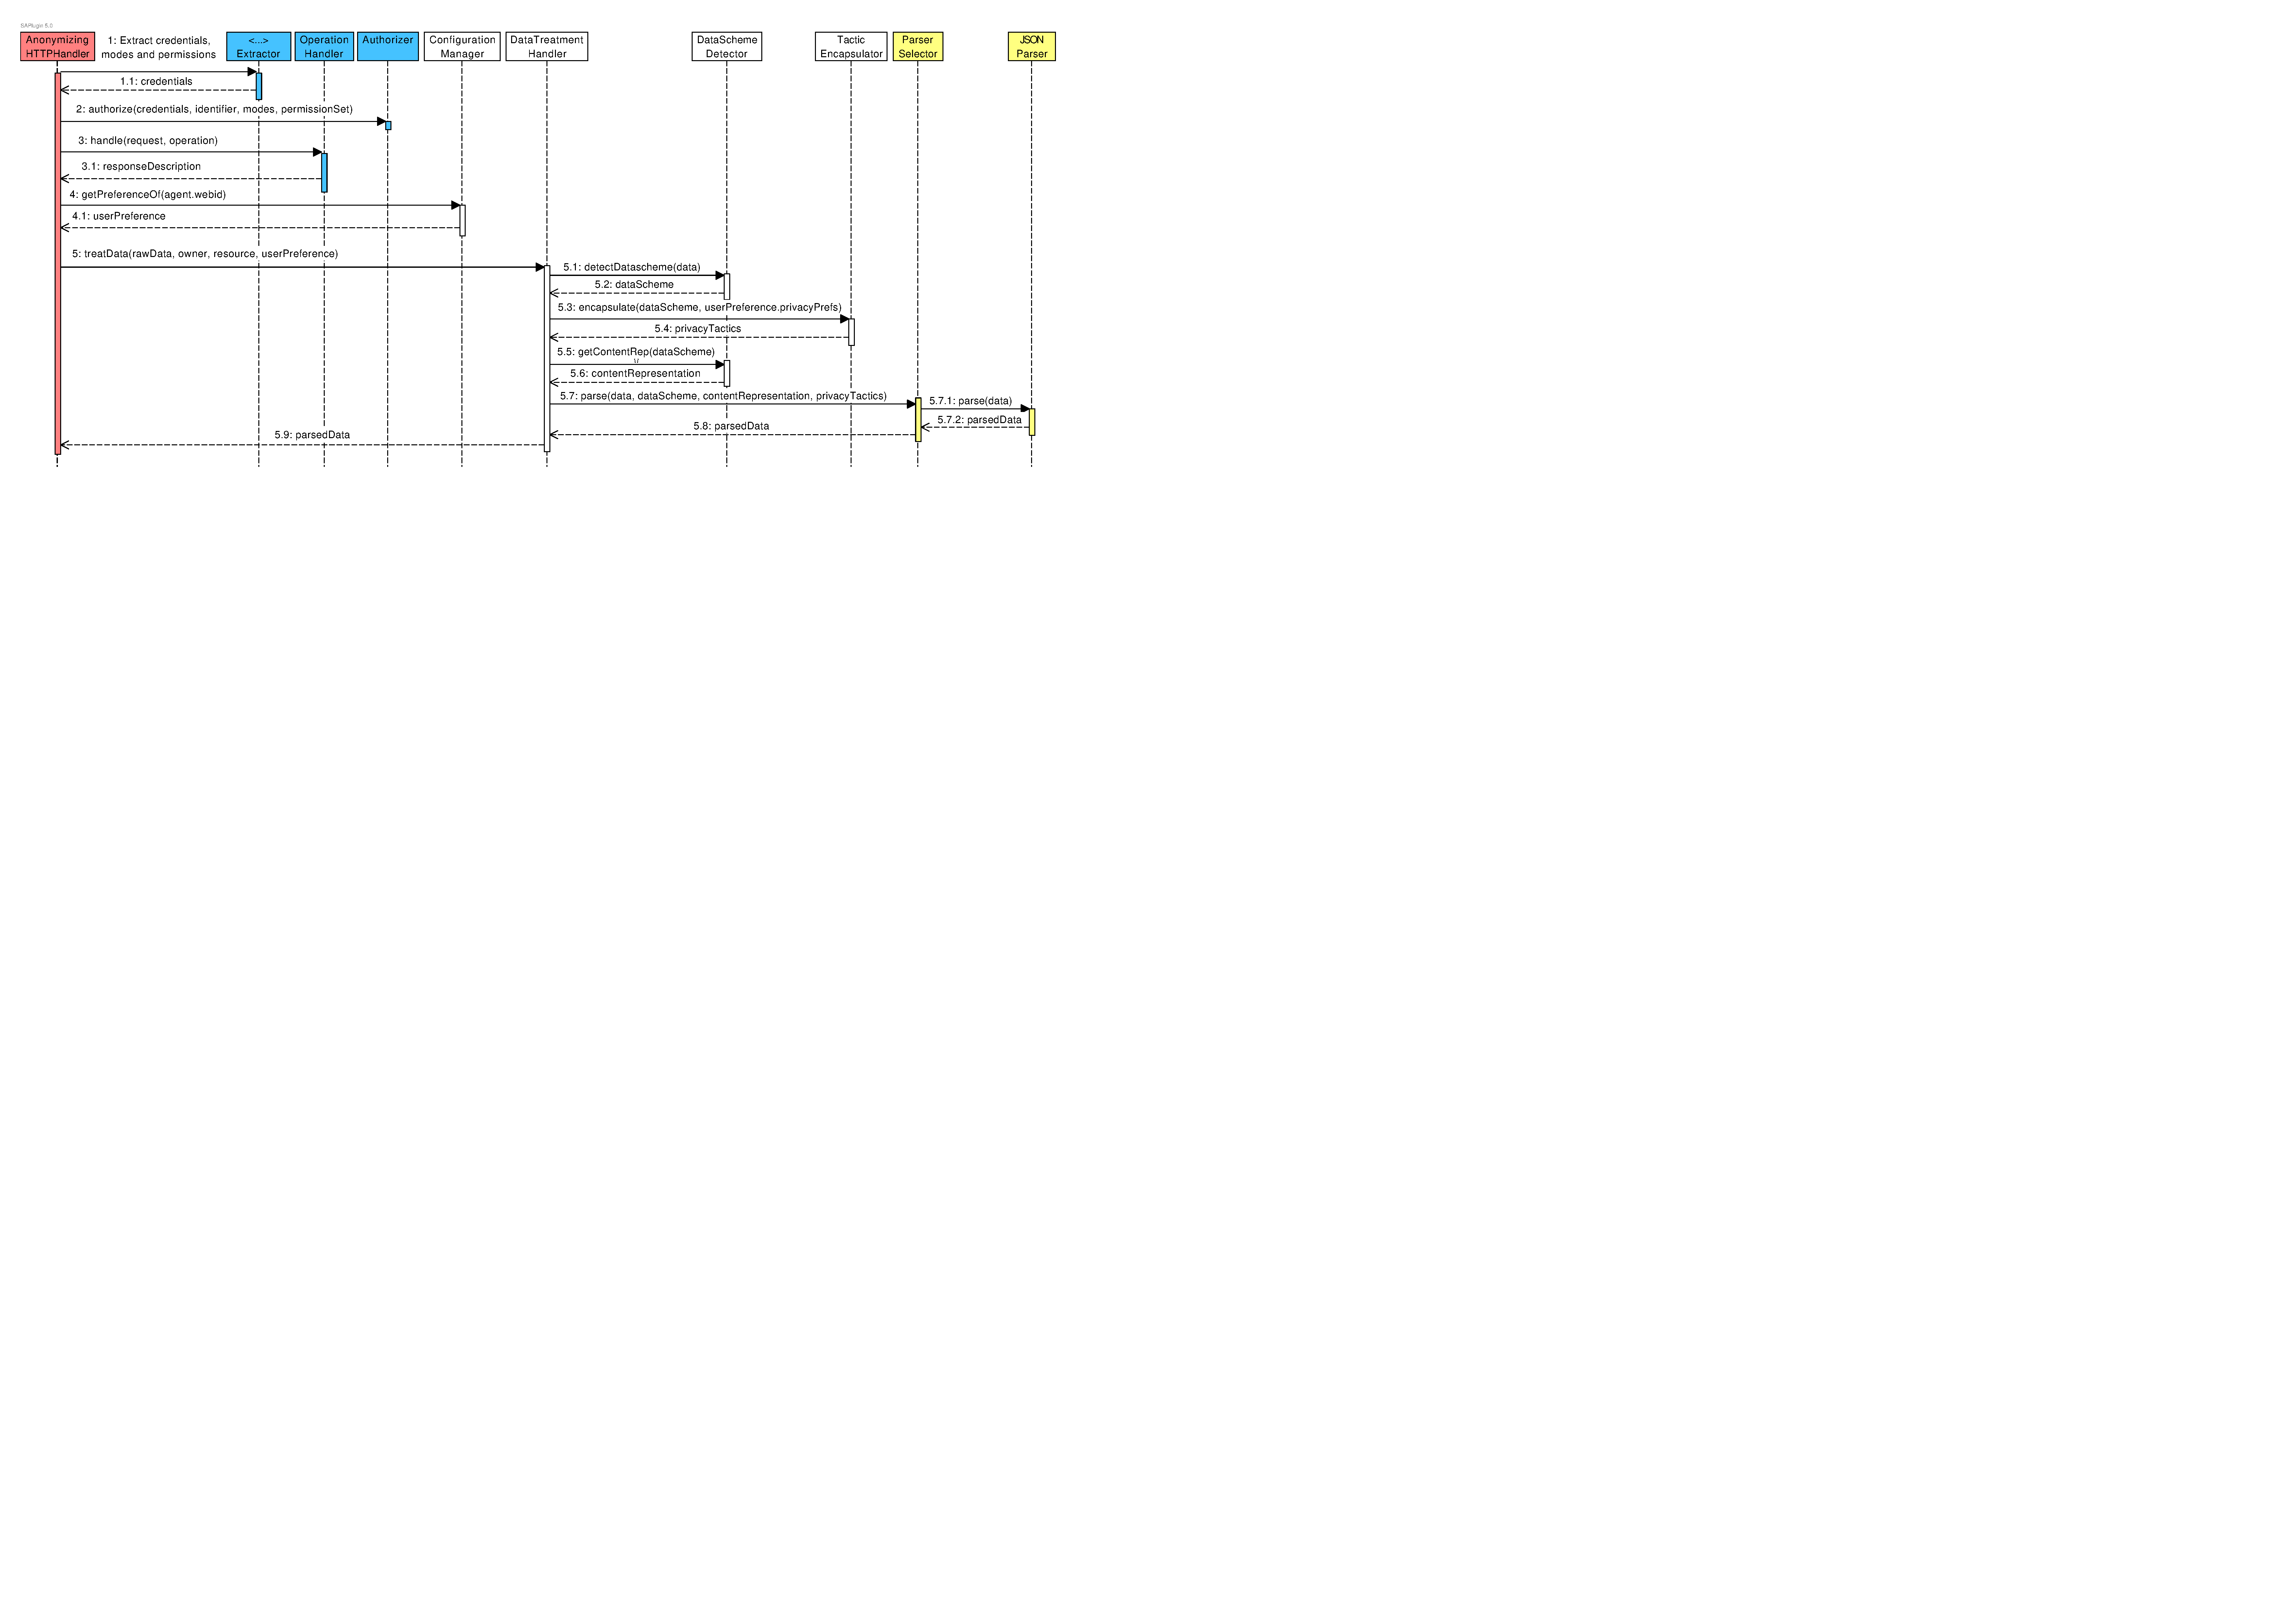
\includegraphics[width=1.0\textwidth]{images/architecture/InteractionDiagram-Rewrite-Flow-PePSA.pdf}
    \caption{Flow of \middleware{} request rewrite}
    \label{fig:pepsa-sequence}
\end{sidewaysfigure}